\documentclass[12pt, letterpaper]{article}
\usepackage[vlined]{algorithm2e}
\usepackage{amsmath}
\usepackage{booktabs}
\usepackage{graphicx}
\usepackage{hyperref}
\usepackage{microtype}

\title{Machine Learning Engineer Nanodegree\\Capstone Report}
\author{Daniel Chao Zhou}
\date{31 December 2019}

\begin{document}

\maketitle

\section{Definition} % (approx. 1-2 pages)

\subsection{Project Overview}

\paragraph{}
The stock market prediction has been identified as a significant practical problem in the economic field. Trading algorithms rather than humans performed over 80\% of trading in the stock market and the FOREX market. In the crypto-currency market, algorithmic trading is also a hot topic among investors. However, timely and accurate prediction of the market is generally regarded as one of the most challenging problems, since the environment is profoundly affected by volatile political-economic factors, such as legislative acts, political unrest, and mass irrational panic.

\paragraph{}
There are many studies regarding algorithmic trading in financial markets based on machine learning, where recurrent neural network (RNN) and reinforcement learning (RL) are being popular in recent years. In this study, a Bitcoin price predictor based on long short-term memory (LSTM, a variant of RNN) is presented.

\subsection{Problem Statement}

\paragraph{}
Given the time-series trading data of a Bitcoin futures contract with each time step indicating one minute, the goal is to build a predictor for the volume-weighted average price (VWAP) of the next minute.

\paragraph{}
In this study, a price predictor based on LSTM will be built.

\subsection{Metrics}

\paragraph{}
The root-mean-square deviation (RMSD) between labels \(y\) and predictions \(\hat y\) will be used to evaluate the performance of both of the benchmark model and the solution model. RMSD is defined as follows,

\begin{align*}
    \mathrm{MSE}(y,\hat y) & :=\frac{1}{N}\sum_i{(y_i-\hat y_i)}^2, \\
    \mathrm{RMSD}(y,\hat y) & :=\sqrt{\mathrm{MSE}(y,\hat y)}.
\end{align*}

For each time step \(t\), the label \(y_t\) is defined as the VWAP of the next time step,

\begin{equation*}
    y_t:=\mathtt{vwap}_{t+1}.
\end{equation*}

\section{Analysis} % (approx. 2-4 pages)

\subsection{Data Exploration}

\paragraph{}
In this study, trading data of BitMEX's XBTZ19 contract, which is a Bitcoin futures contract being traded around the clock from 16 June to 27 December 2019, will be used to train and test the predictor. The dataset could be fetched from BitMEX's official API without charge of fee.\footnote{The API concerned with the desired data is documented at \url{https://www.bitmex.com/api/explorer/\#!/Trade/Trade_getBucketed}}

\paragraph{}
The dataset is a table that each row indicates one minute and each column indicates a specific data as described in Table~\ref{table:column-header}. Note that \texttt{open} is not defined as the price of the first trade in the specific time step, which is an unconventional definition and does not apply to other data sources.

\begin{table}
    \centering
    \begin{tabular}{ll}
        \toprule
        \texttt{high} & highest price \\
        \texttt{low} & lowest price \\
        \texttt{close} & price of the last trade \\
        \texttt{open} & \texttt{close} of the last time step \\
        \texttt{vwap} & volume-weighted average price (VWAP) \\
        \texttt{foreignNotional} & traded amount in units of US dollar \\
        \texttt{homeNotional} & traded amount in units of Bitcoin \\
        \texttt{trades} & number of trades \\
        \texttt{volume} & alias of \texttt{foreignNotional} \\
        \bottomrule
    \end{tabular}
    \caption{Column header semantics}%
    \label{table:column-header}
\end{table}

\paragraph{}
The dataset is formulated as \( \{x_t|t=1,2,\dots,T\} \), where \(x_t\) is a vector of the data in minute \(t\), such that \(x_t=(\mathtt{open}_t,\mathtt{high}_t,\mathtt{low}_t,\mathtt{close}_t,\mathtt{vwap}_t,\dots)\). A small sample and some basic statistics are shown in Table~\ref{table:sample} and Table~\ref{table:statistics}.

\begin{table}
    \resizebox{\textwidth}{!}{
    \begin{tabular}{l*8r}
        \toprule
        & open & high & low & close & vwap & foreignNotional & homeNotional & trades \\
        \midrule
        2019--06--14 08:31 & NaN & NaN & NaN & NaN & NaN & 0 & 0.000000 & 0 \\
        2019--06--14 08:32 & NaN & NaN & NaN & NaN & NaN & 0 & 0.000000 & 0 \\
        2019--06--14 08:33 & 8500.00 & 8500.00 & 8260.00 & 8260.00 & 8262.4143 & 201 & 0.024328 & 3 \\
        2019--06--14 08:34 & 8260.00 & 8390.00 & 8308.00 & 8308.00 & 8325.0083 & 13110 & 1.574852 & 7 \\
        2019--06--14 08:35 & 8308.00 & 8390.00 & 8319.50 & 8336.50 & 8322.9297 & 13200 & 1.585986 & 5 \\
        2019--06--14 08:36 & 8336.50 & 8317.50 & 8317.50 & 8317.50 & 8317.5000 & 10200 & 1.226346 & 3 \\
        2019--06--14 08:37 & 8317.50 & 8327.50 & 8327.50 & 8327.50 & 8328.0000 & 500 & 0.060040 & 1 \\
        2019--06--14 08:38 & 8327.50 & 8366.50 & 8362.50 & 8362.50 & 8365.4007 & 4001 & 0.478290 & 5 \\
        \dots & \dots & \dots & \dots & \dots & \dots & \dots & \dots & \dots \\
        2019--12--27 11:54 & 7151.00 & 7155.50 & 7135.00 & 7137.50 & 7149.4960 & 632224 & 88.434680 & 62 \\
        2019--12--27 11:55 & 7137.50 & 7149.50 & 7137.50 & 7149.00 & 7141.3269 & 60153 & 8.423772 & 44 \\
        2019--12--27 11:56 & 7149.00 & 7142.00 & 7140.50 & 7141.50 & 7140.8169 & 407108 & 57.015170 & 34 \\
        2019--12--27 11:57 & 7141.50 & 7149.50 & 7141.00 & 7141.50 & 7141.3269 & 325738 & 45.615289 & 22 \\
        2019--12--27 11:58 & 7141.50 & 7150.00 & 7141.50 & 7150.00 & 7149.4960 & 390967 & 54.686307 & 31 \\
        2019--12--27 11:59 & 7150.00 & 7150.00 & 7141.00 & 7148.50 & 7142.8571 & 540701 & 75.700246 & 30 \\
        2019--12--27 12:00 & 7148.50 & 7148.50 & 7138.24 & 7138.24 & 7138.7778 & 41934166 & 5874.536073 & 59 \\
        2019--12--27 12:01 & 7138.24 & 7138.24 & 7138.24 & 7138.24 & NaN & 0 & 0.000000 & 0 \\
        \bottomrule
    \end{tabular}}
    \caption{Head and tail part of the dataset}%
    \label{table:sample}
\end{table}

\begin{table}
    \resizebox{\textwidth}{!}{
    \begin{tabular}{l*8r}
        \toprule
        & open & high & low & close & vwap & foreignNotional & homeNotional & trades \\
        \midrule
        count & 282449.00 & 282449.00 & 282449.00 & 282449.00 & 243964.00 & 2.82e+05 & 282451.00 & 282451.00 \\
        mean & 9499.88 & 9502.96 & 9496.68 & 9499.87 & 9558.33 & 3.69e+04 & 3.94 & 23.43 \\
        std & 1621.16 & 1622.74 & 1619.51 & 1621.17 & 1632.99 & 1.37e+05 & 16.63 & 46.27 \\
        min & 6438.00 & 6443.50 & 6431.00 & 6438.00 & 6432.52 & 0.00e+00 & 0.00 & 0.00 \\
        25\% & 8158.00 & 8159.50 & 8157.00 & 8158.00 & 8180.62 & 6.05e+02 & 0.06 & 2.00 \\
        50\% & 9542.50 & 9546.00 & 9540.00 & 9542.50 & 9589.56 & 7.33e+03 & 0.77 & 10.00 \\
        75\% & 10616.50 & 10619.50 & 10614.00 & 10616.50 & 10656.43 & 3.20e+04 & 3.36 & 26.00 \\
        max & 14600.00 & 14600.00 & 14539.00 & 14600.00 & 14547.57 & 4.19e+07 & 5874.53 & 1529.00 \\
        \bottomrule
    \end{tabular}}
    \caption{Basic statistics of the dataset}%
    \label{table:statistics}
\end{table}

\subsection{Exploratory Visualization}

\paragraph{}
The VWAP and volume of the dataset are shown in Figure~\ref{fig:dataset}.

\begin{figure}
    \centering
    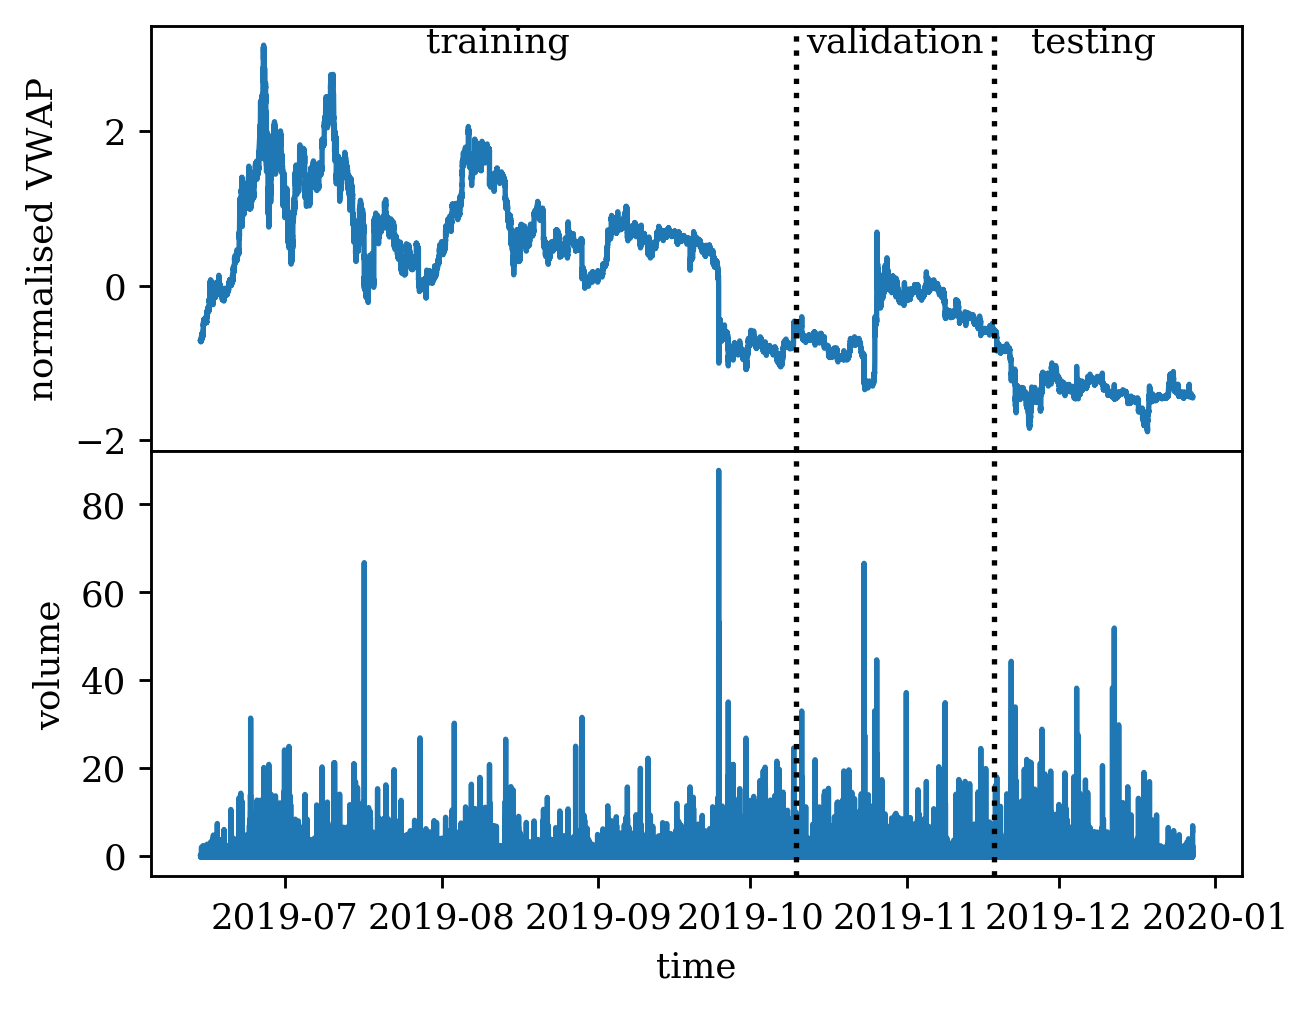
\includegraphics[width=\textwidth]{figures/dataset.png}
    \caption{VWAP and volume of the dataset}%
    \label{fig:dataset}
\end{figure}

\subsection{Algorithms and Techniques}

\paragraph{}
The solution model consists of one LSTM layer and one linear layer. The LSTM layer is formally formulated as follows:

\begin{align*}
    i_t & =\sigma\left(W_{ii}x_t+b_{ii}+W_{hi}h_{(t-1)}+b_{hi}\right), \\
    f_t & =\sigma\left(W_{if}x_t+b_{if}+W_{hf}h_{(t-1)}+b_{hf}\right), \\
    g_t & =\tanh\left(W_{ig}x_t+b_{ig}+W_{hg}h_{(t-1)}+b_{hg}\right), \\
    o_t & =\sigma\left(W_{io}x_t+b_{io}+W_{ho}h_{(t-1)}+b_{ho}\right), \\
    c_t & =f_t*c_{(t-1)}+i_t*g_t, \\
    h_t & =o_t*\tanh(c_t).
\end{align*}

where \(h_t\) is the hidden state at time \(t\), \(c_t\) is the cell state at time \(t\), \(x_t\) is the input at time \(t\), and \(i_t\), \(f_t\), \(g_t\), \(o_t\) are the input, forget, cell, and output gates, respectively. \(\sigma \) is the sigmoid function, and \(*\) is the Hadamard product.

\paragraph{}
Moreover, the tunable parameters are listed as follows:

\begin{enumerate}
    \item \texttt{hidden\_dim}\quad the number of dimension of the hidden layer between the LSTM and the linear network;
    \item \texttt{dropout}\quad the dropout regularisation parameter for the LSTM network;
    \item \texttt{lr}\quad the learning rate;
    \item \texttt{batch\_size}\quad the number of rows for each batch; and
    \item \texttt{n\_epochs}\quad the number of epochs.
\end{enumerate}

\subsection{Benchmark}

\paragraph{}
The benchmark model consists of two linear regression layers:

\begin{align*}
    h & =\mathrm{ReLU}\left(xA_1+b_1\right), \\
    \hat y & =hA_2+b_2.
\end{align*}

\section{Methodology} % (approx. 3-5 pages)

\subsection{Data Preprocessing}

\paragraph{}
Data preprocessing steps are listed as follows.

\begin{enumerate}
    \item \textbf{Crawling} Since new data are generating every minute before the futures expires, new rows could be fetched from the data source. The crawler should be able to handle locally cached data and progressively persisting new data.
    \item \textbf{Column dropping} Columns \texttt{open} and \texttt{volume} do not provide new information to the rest part and are consequently dropped.
    \item \textbf{Null filling} For time steps that do not contain any trades, the corresponding \texttt{vwap} columns are null. These items will be propagated with last valid observations.
    \item \textbf{Feature engineering} Moving average convergence/divergence (MACD) with the short period of 12 and the long period of 26, and relative strength index (RSI) with the timeframe of 14, are calculated and appended as extra columns for consequent processing.
    \item \textbf{Normalisation} All features will be normalised.
    \item \textbf{Labelling} Each row will be labelled a learning target. The learning target has different definitions in the initial and final solution, which will be illustrated in Subsection~\ref{sec:refinement}.
    \item \textbf{Splitting} The entire dataset will be split without shuffling into three consecutive parts for training, validation, and testing, while the lengths proportionate to 6:2:2. Individually, their ranges are listed in Table~\ref{table:split}.
\end{enumerate}

\begin{table}
    \centering
    \begin{tabular}{lrr}
        \toprule
                   &         from &           to \\
        \midrule
        training   & 2019--06--14 & 2019--10--09 \\
        validation & 2019--10--10 & 2019--11--17 \\
        testing    & 2019--11--18 & 2019--12--27 \\
        \bottomrule
    \end{tabular}
    \caption{Dataset splitting}%
    \label{table:split}
\end{table}

\subsection{Implementation}

\paragraph{}
The LSTM model was implemented with PyTorch's builtin \texttt{torch.nn.LSTM} class. Besides, the training steps are listed as follows.

\begin{algorithm}
    load preprocessed training and validation data into CUDA device\;
    load parameters\;
    initialise model\;
    initialise loss function \texttt{torch.nn.MSELoss}\;
    initialise optimiser \texttt{torch.optim.Adam}\;
    initialise scheduler \texttt{torch.optim.lr\_scheduler.StepLR}\;
    \ForEach{epoch}{
        split training data into batchs\;
        initialise hidden states and cell states with zero vectors\;
        \ForEach{training batch}{
            clear all gradients\;
            execute forward propagation, get estimator, and update hidden/cell states\;
            get loss value from the estimator\;
            execute backpropagation and update the model\;
        }
        get loss value of the validation data\;
    }
\end{algorithm}

\subsection{Refinement}\label{sec:refinement}

\paragraph{}
In the initial solution, the learning target is the label \(y\), i.e.\ the VWAP of the next time step, i.e.

\begin{equation*}
    \hat y_t=f(x_t)=\mathtt{vwap}_{t+1}+\varepsilon_t,
\end{equation*}

where \(f(\cdot)\) is the LSTM model and \(\varepsilon_n\) is the residual. However, in this solution, a high bias is observed on the testing dataset (as shown in Figure~\ref{fig:pred1}). Since the price does not vary significantly in one minute, using the model to estimate the price change in one minute could reduce the bias, which leads to the final solution.

\paragraph{}
In the final solution, the learning target is defined as the difference of the logarithm of the VWAP between this time step and the next, i.e.

\begin{align*}
    f(x_t) & =\log(\mathtt{vwap}_{t+1})-\log(\mathtt{vwap}_t)+\varepsilon_t, \\
    \hat y_t & =\mathtt{vwap}_t\exp(f(x_t))=\mathtt{vwap}_{t+1}\exp(\varepsilon_t).
\end{align*}

Even though the estimation \(\hat y\) is more vulnerable to a higher residual than the former solution, both bias and variance are reduced in the experiment results.

\paragraph{}
In the following sections, these two solutions described above will be named Solution I and Solution II\@.

\section{Results} % (approx. 2-3 pages)

\subsection{Model Evaluation and Validation}

\paragraph{}
Since the dataset, containing 282452 minutes/rows, is big enough, and the test data was not used to train or tune the model, it could be concluded that the model is robust enough to estimate unseen data.

\subsection{Justification}

\paragraph{}
The RMSD losses of three models w.r.t.\ three datasets are listed in Table~\ref{table:loss}, which illustrates that the final solution (Solution II) overperforms the benchmark significantly on the entire dataset.

\begin{table}
    \centering
    \begin{tabular}{llr}
        \toprule
        Model       & Dataset    &   RMSD \\
        \midrule
                    & training   & 209.53 \\
        Benchmark   & validation & 107.05 \\
                    & testing    & 125.28 \\
        \midrule
                    & training   & 147.93 \\
        Solution I  & validation & 110.03 \\
                    & testing    & 476.31 \\
        \midrule
                    & training   &  11.96 \\
        Solution II & validation &   6.98 \\
                    & testing    &   5.53 \\
        \bottomrule
    \end{tabular}
    \caption{Loss}%
    \label{table:loss}
\end{table}

\paragraph{}
The comparison between ground truth and predictions w.r.t.\ the linear model as a benchmark and two LSTM based solution models discussed in Subsection~\ref{sec:refinement}, are shown in Figure~\ref{fig:pred0},\ \ref{fig:pred1}, and\ \ref{fig:pred2}. Based on these three figures we can conclude that

\begin{enumerate}
    \item The benchmark model performs poorly when price change rapidly, as the orange curve diverges from the blue curve at peaks and troughs;
    \item Solution I shows a lower variance than the linear model, but also a high bias in the testing dataset; and
    \item Solution II produces an unbiased and efficient estimation on the entire dataset, as the blue curve is almost perfectly covered by orange.
\end{enumerate}

\begin{figure}
    \centering
    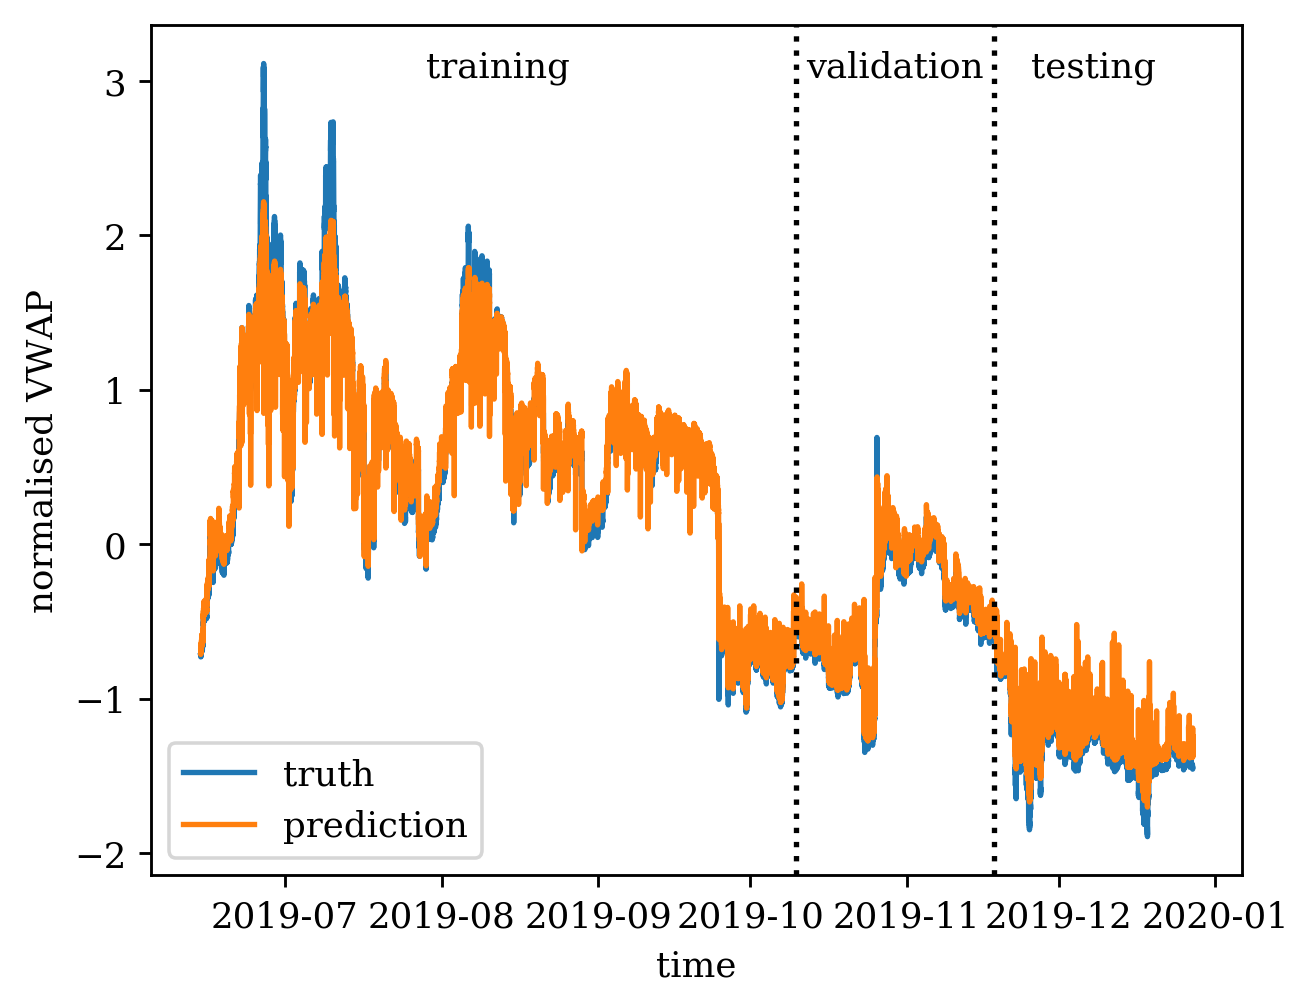
\includegraphics{figures/pred_linear.png}
    \caption{Prediction of Benchmark}%
    \label{fig:pred0}
\end{figure}

\begin{figure}
    \centering
    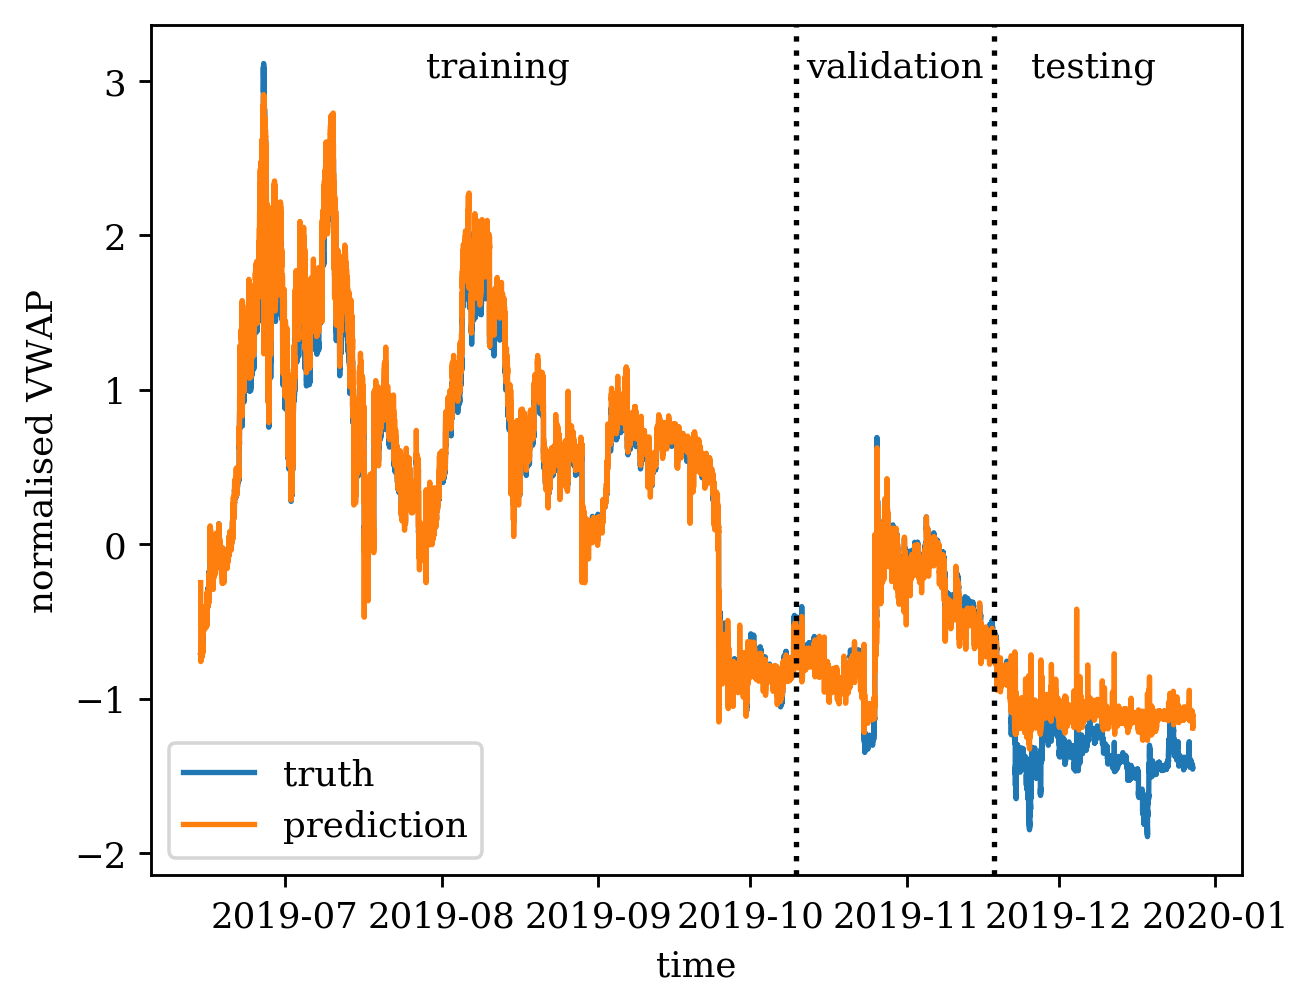
\includegraphics{figures/pred_lstm.png}
    \caption{Prediction of Solution I}%
    \label{fig:pred1}
\end{figure}

\begin{figure}
    \centering
    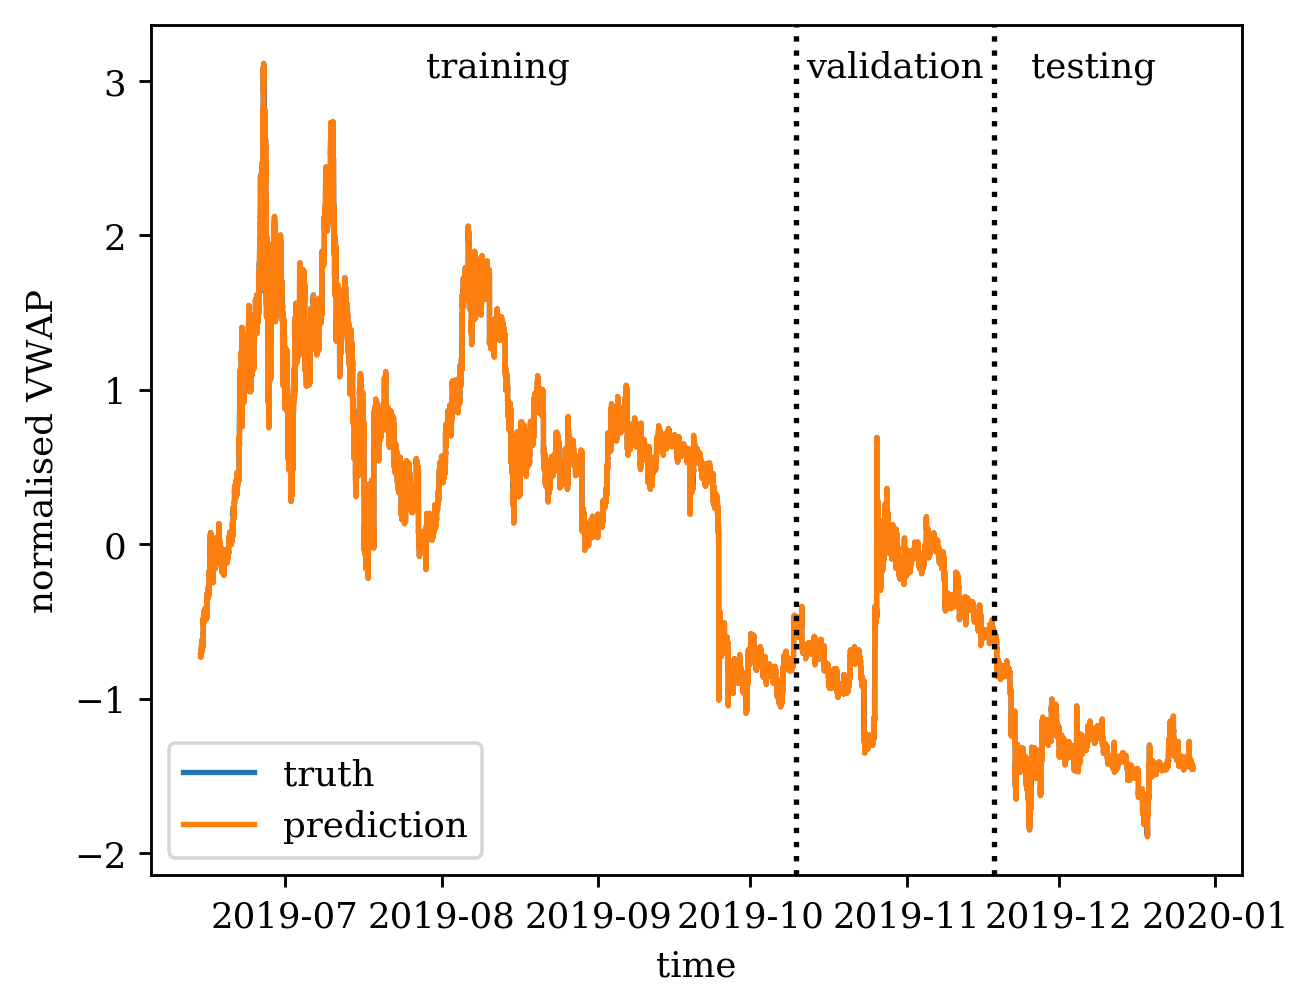
\includegraphics{figures/pred_lstmratio.png}
    \caption{Prediction of Solution II}%
    \label{fig:pred2}
\end{figure}

\section{Conclusion}

\subsection{Reflection}

\paragraph{}
In this study, an LSTM-based predictor was built to estimate VWAP of Bitcoin futures contract using history trading data. The model does not estimate VWAP itself, but the logarithm of VWAP change. Empirically, the RMSD between estimated and real VWAP on the test data is 5.53, which significantly overperforms the benchmark model, whose RMSD is 125.28.

\paragraph{}
However, even though the estimated price almost overlaps with the real price on Figure~\ref{fig:pred2}, further analysis is required to conclude whether this predictor is precise enough to serve as a trading agent that beats the market.

\subsection{Improvement}

\paragraph{}
The trading data in financial markets is infamous to have a bad signal-noise-ratio. More data sources outside the market, such as Google Index of the keyword ``Bitcoin'', sentiment analysis of the Bitcoin channel on Reddit, could significantly improve the solution of this study.

\paragraph{}
Moreover, a price predictor could be ensembled with a trading policy and yields a trading agent. The trading policy could be some simple rules or a complex mathematical model. Otherwise, a reinforcement learning model is also possible to serve as a trading agent.

\end{document}
